We run the graphMiner code that includes k-core algorithm on WiKi-Vote and soc-Epinions1 from SNAP and report the results.

\subsection{radii}
Radius means that for every node r, find the node with longest distance from this distance. 
Namely, the max number of edge between two nodes.
Below we draw the distance histogram of the number of nodes that has distance r.

\begin{figure}[H]
\begin{center}
\begin{tabular}{cc}
     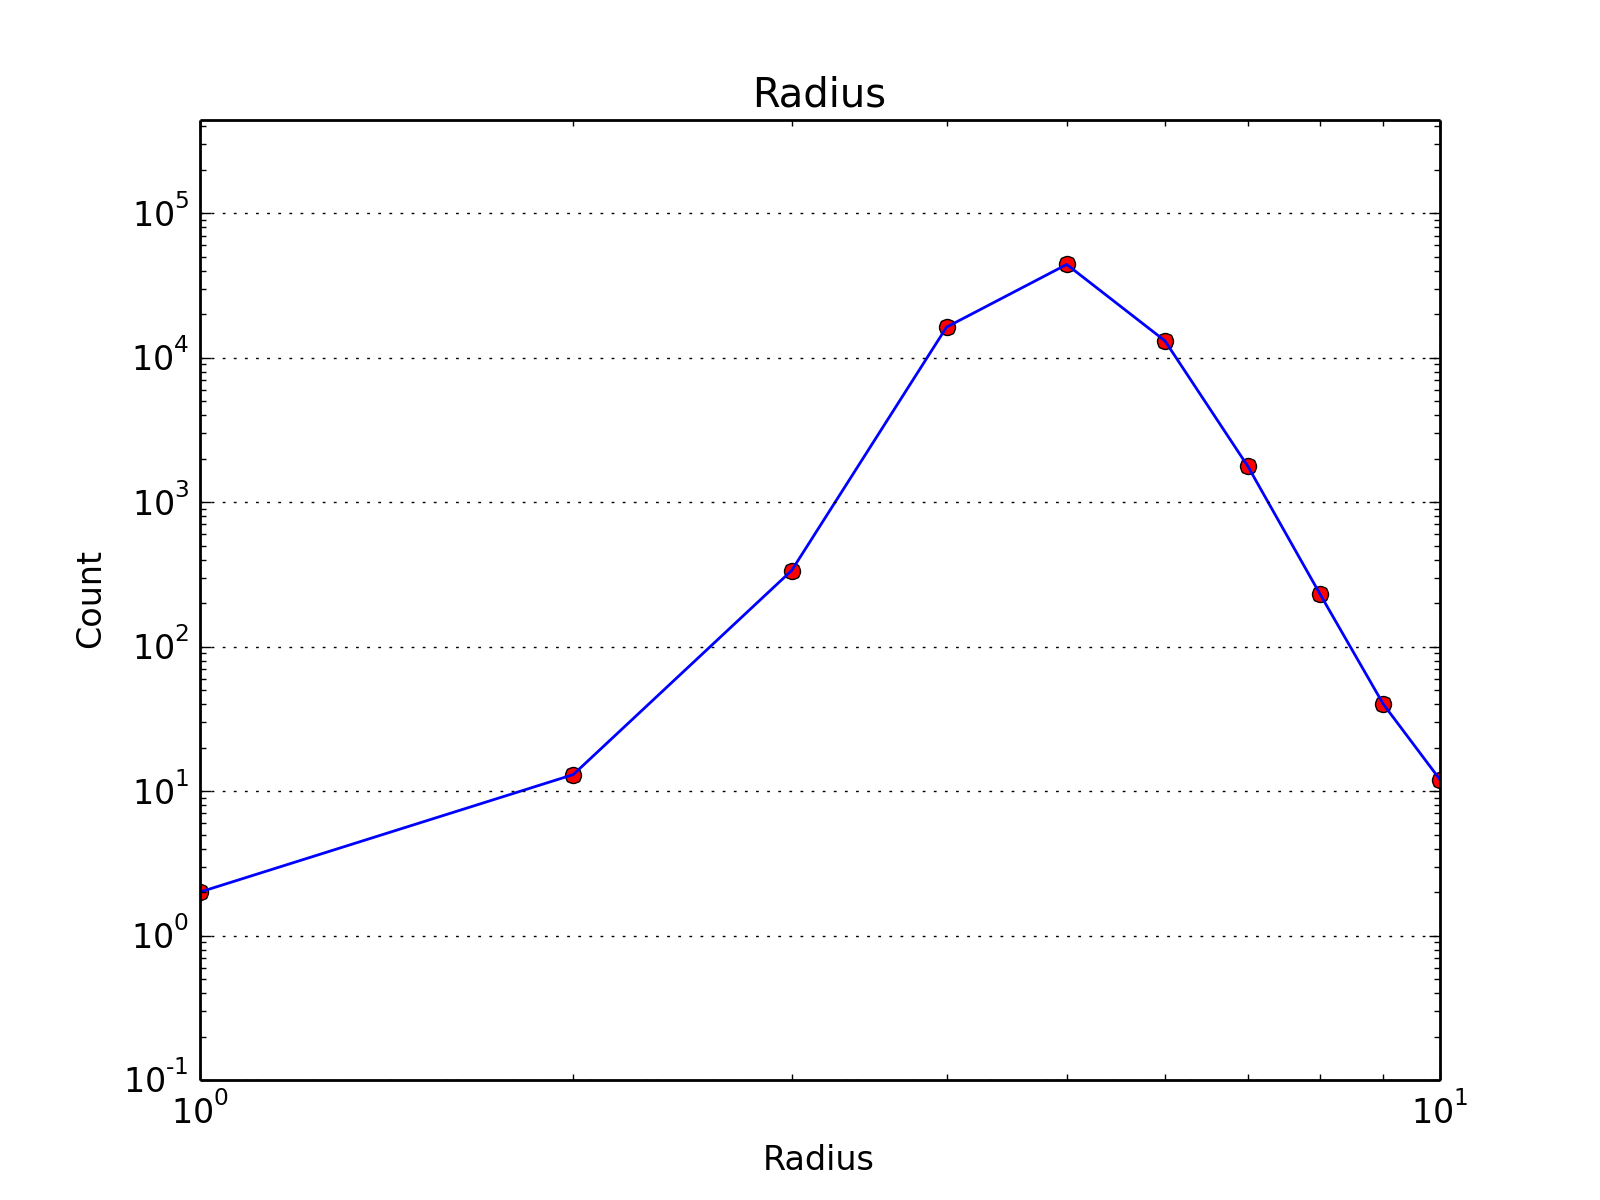
\includegraphics[width=0.5\textwidth]{FIG/Radiusoutput_soc-Epinions1.png} 
     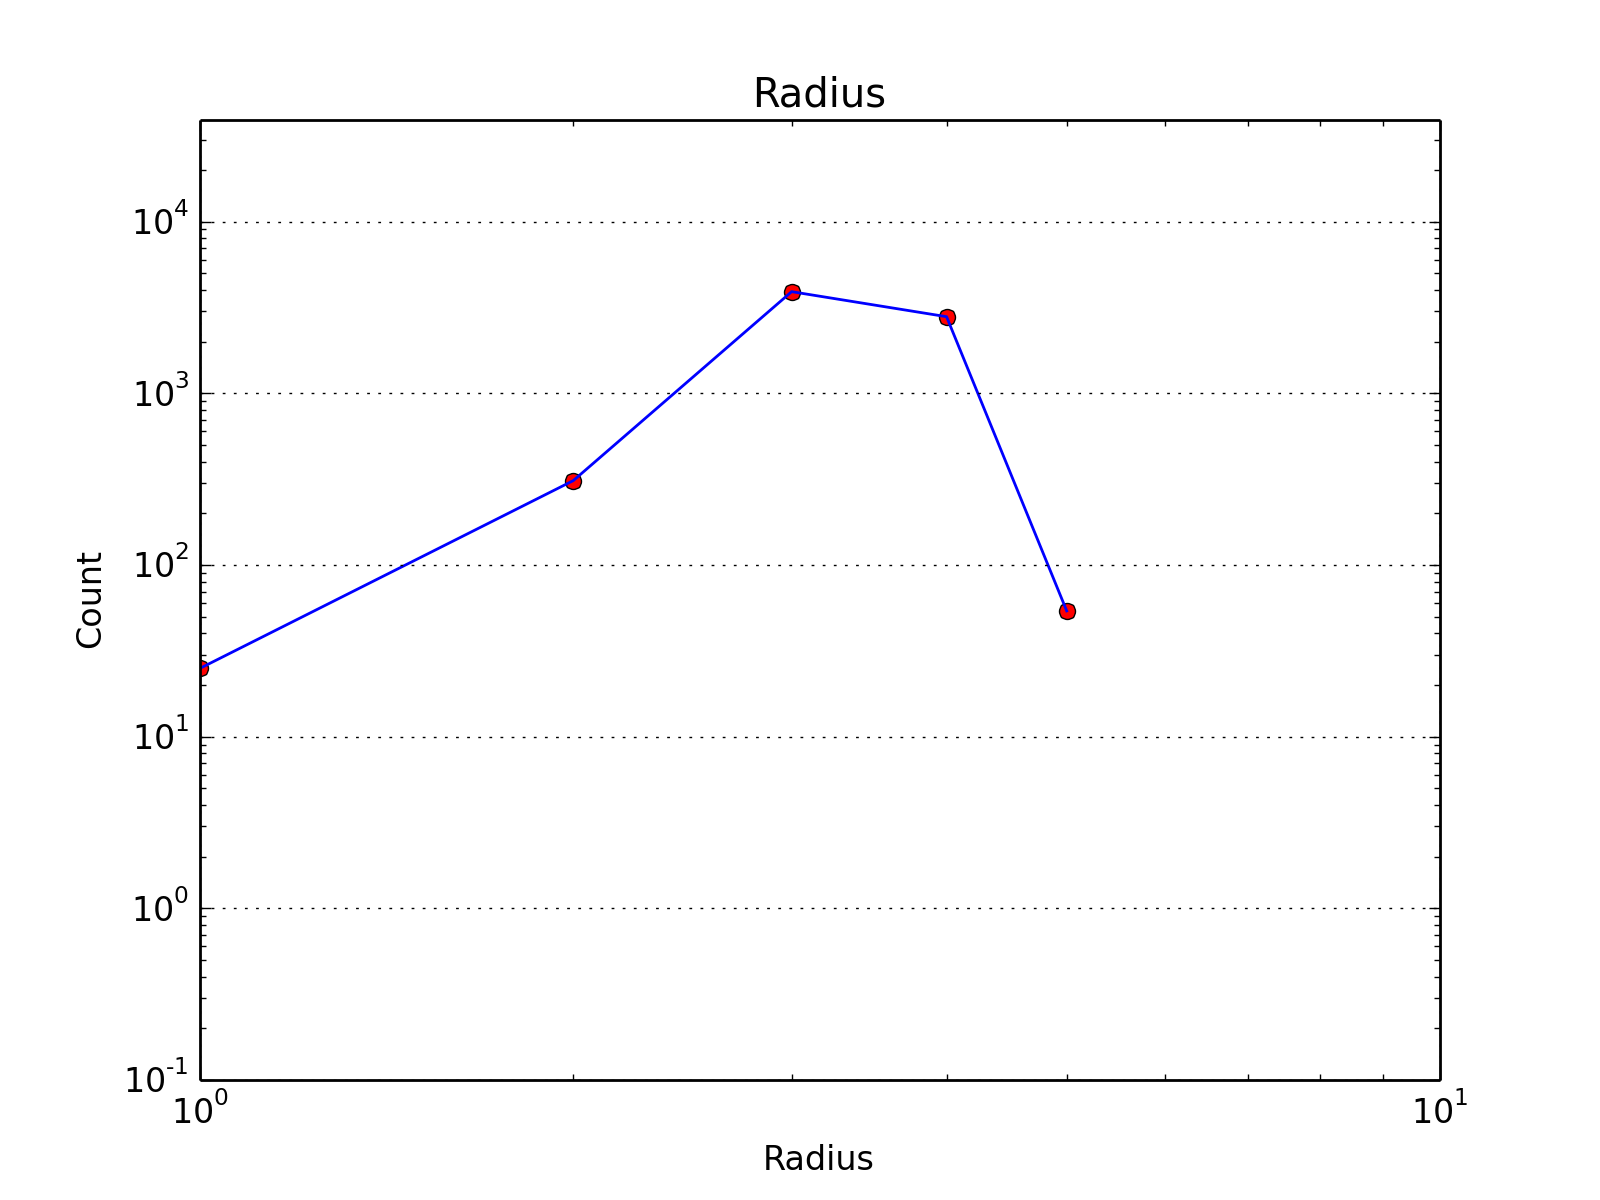
\includegraphics[width=0.5\textwidth]{FIG/Radiusoutput_wiki-Vote.png} 
\end{tabular}
\caption{Radius of soc(left) and Wiki(right)}
\label{fig:results}
\end{center}
\end{figure}

\subsection{eigenvalues and eigenvectors}

The graph could be represented as a matrix, and the eigenvalue and its eigenvector has a special meaning that could indicate the features of the graph. We get the Eigenvalue and eigenvectors using QR decomposition.

SOC:
Eigen Value:
	1,241.29698881924
	2,18.8603144039429
	3,-13.5331106496658
Eigen Vector
	7115*4 vectors

WIKI:
	(1, 148.091823802481)
	(2, -21.9191359313477)
	(3, 5.77260254552437)
Eigen Vector:
	75879*3 vectors


\subsection{Node degree}

We view these graph as undirected graph. This is just a histogram of the degree and its number on log space. The results are as follows:

\begin{figure}[H]
\begin{center}
\begin{tabular}{cc}
     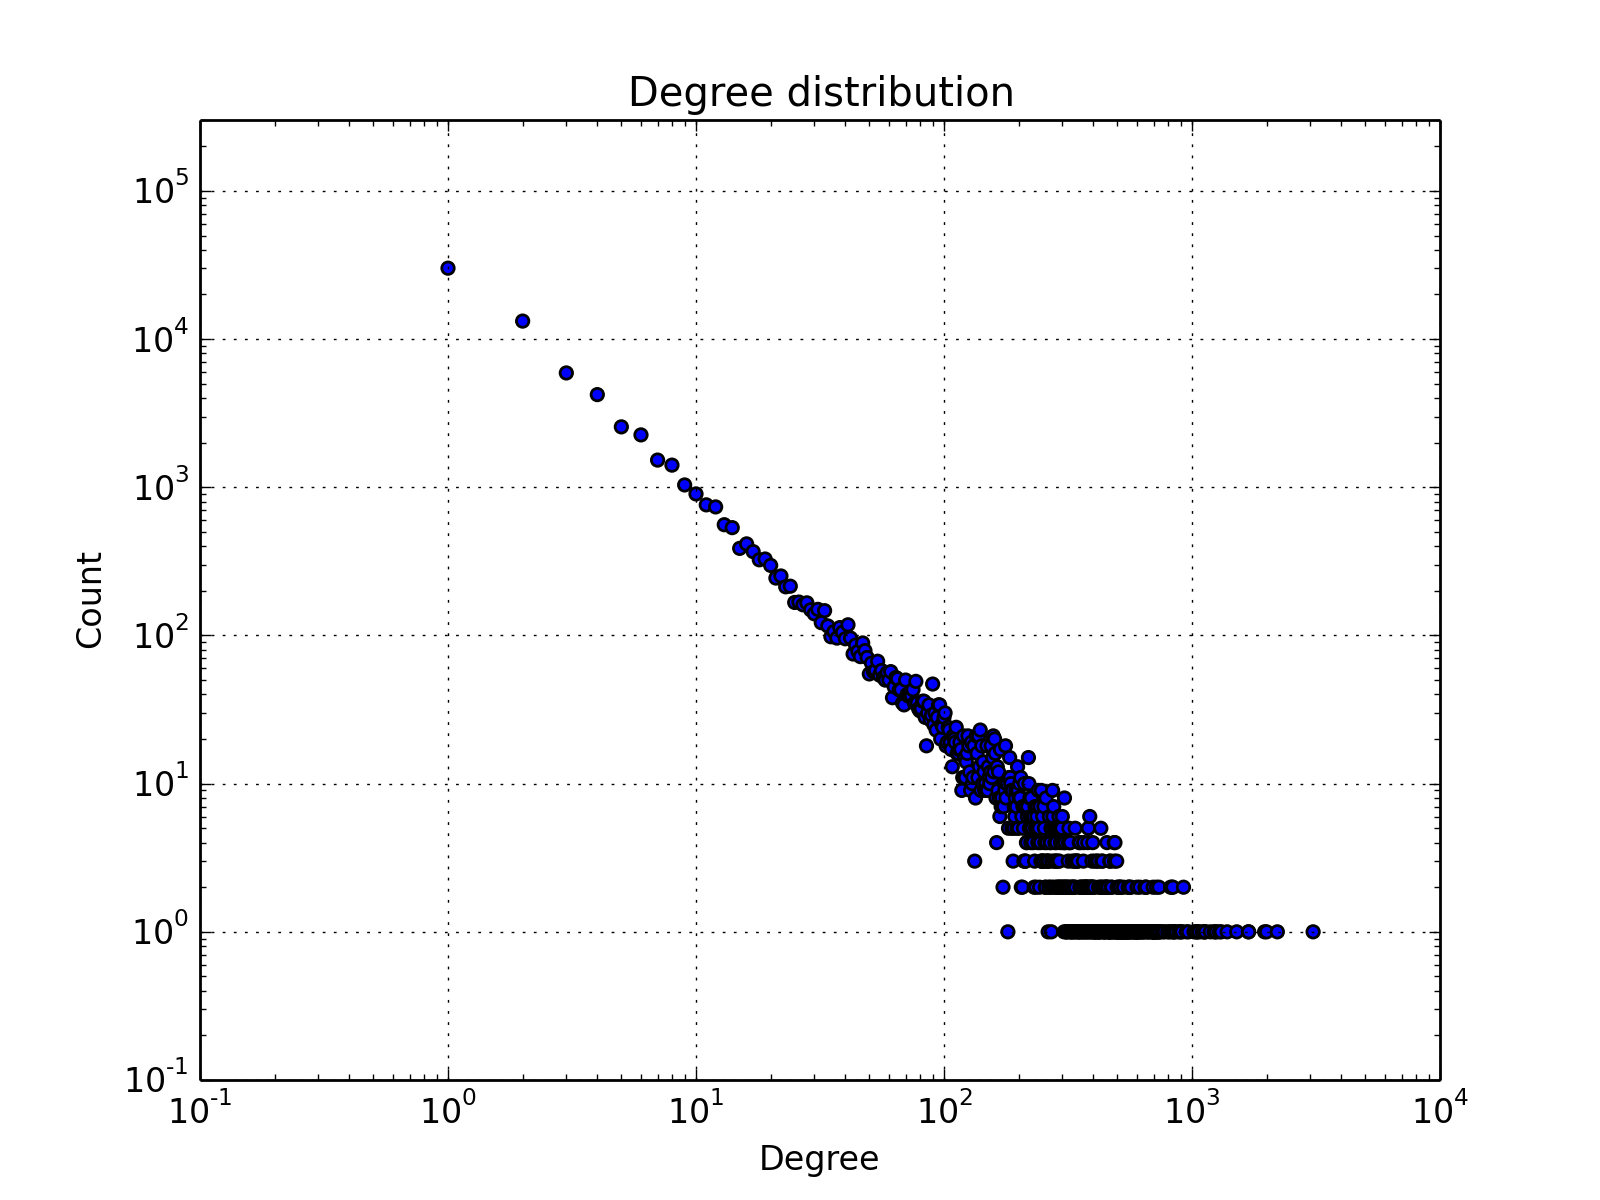
\includegraphics[width=0.5\textwidth]{FIG/DegreeDistoutput_soc-Epinions1.png} 
     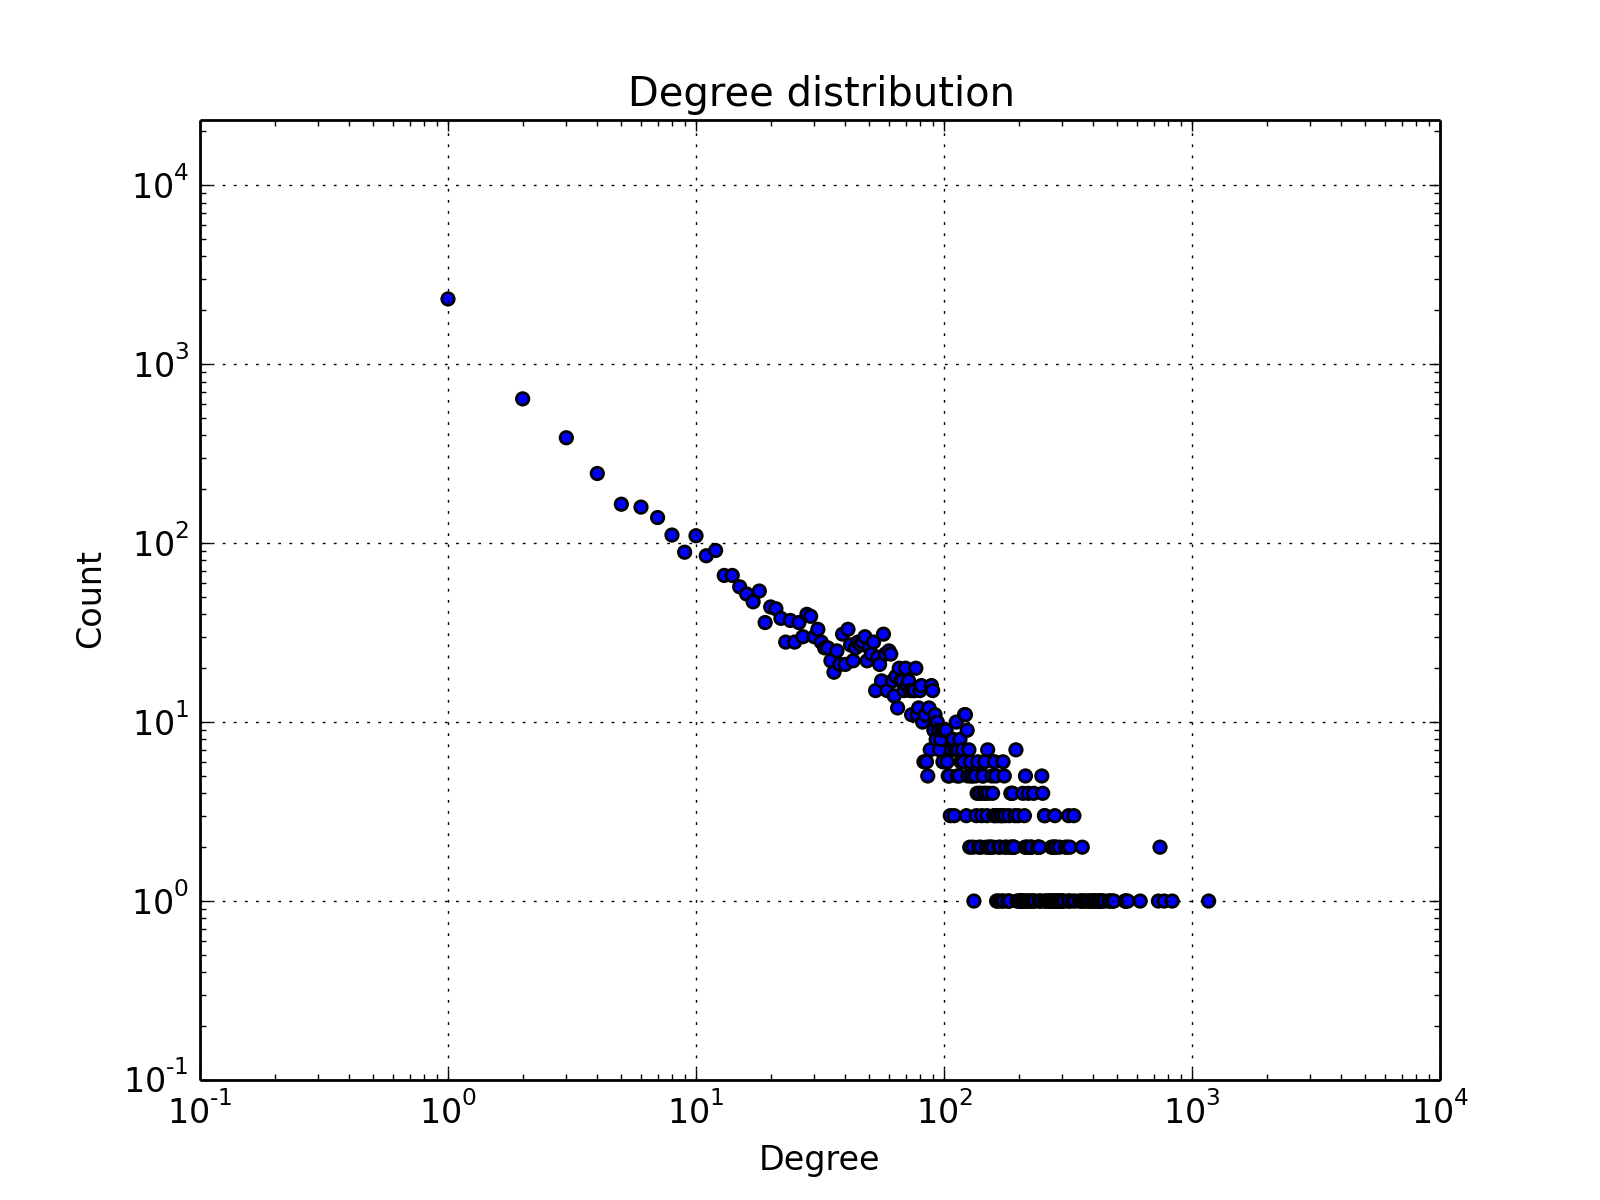
\includegraphics[width=0.5\textwidth]{FIG/DegreeDistoutput_wiki-Vote.png} 
\end{tabular}
\caption{Degree of soc(left) and Wiki(right)}
\label{fig:results}
\end{center}
\end{figure}

\subsection{PageRank}

We can plot PageRank in log space:

\begin{figure}[H]
\begin{center}
\begin{tabular}{cc}
     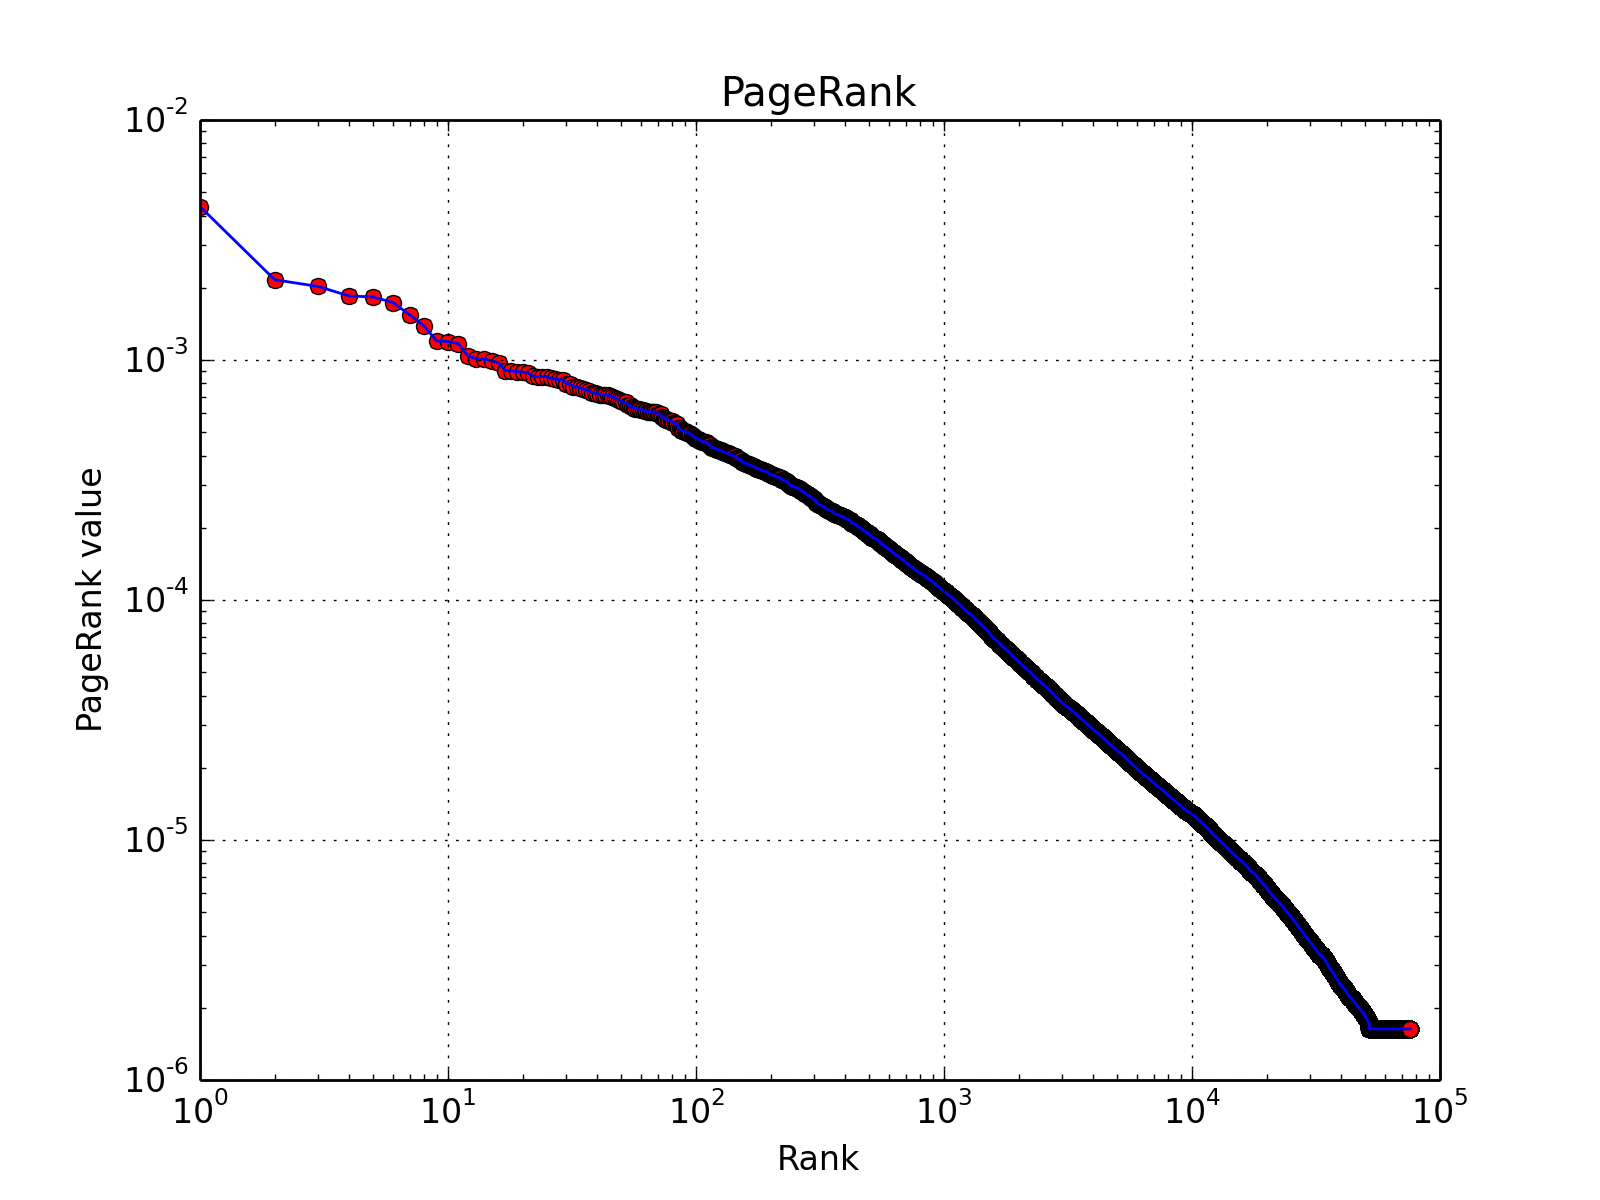
\includegraphics[width=0.5\textwidth]{FIG/pageRankoutput_soc-Epinions1.png} 
     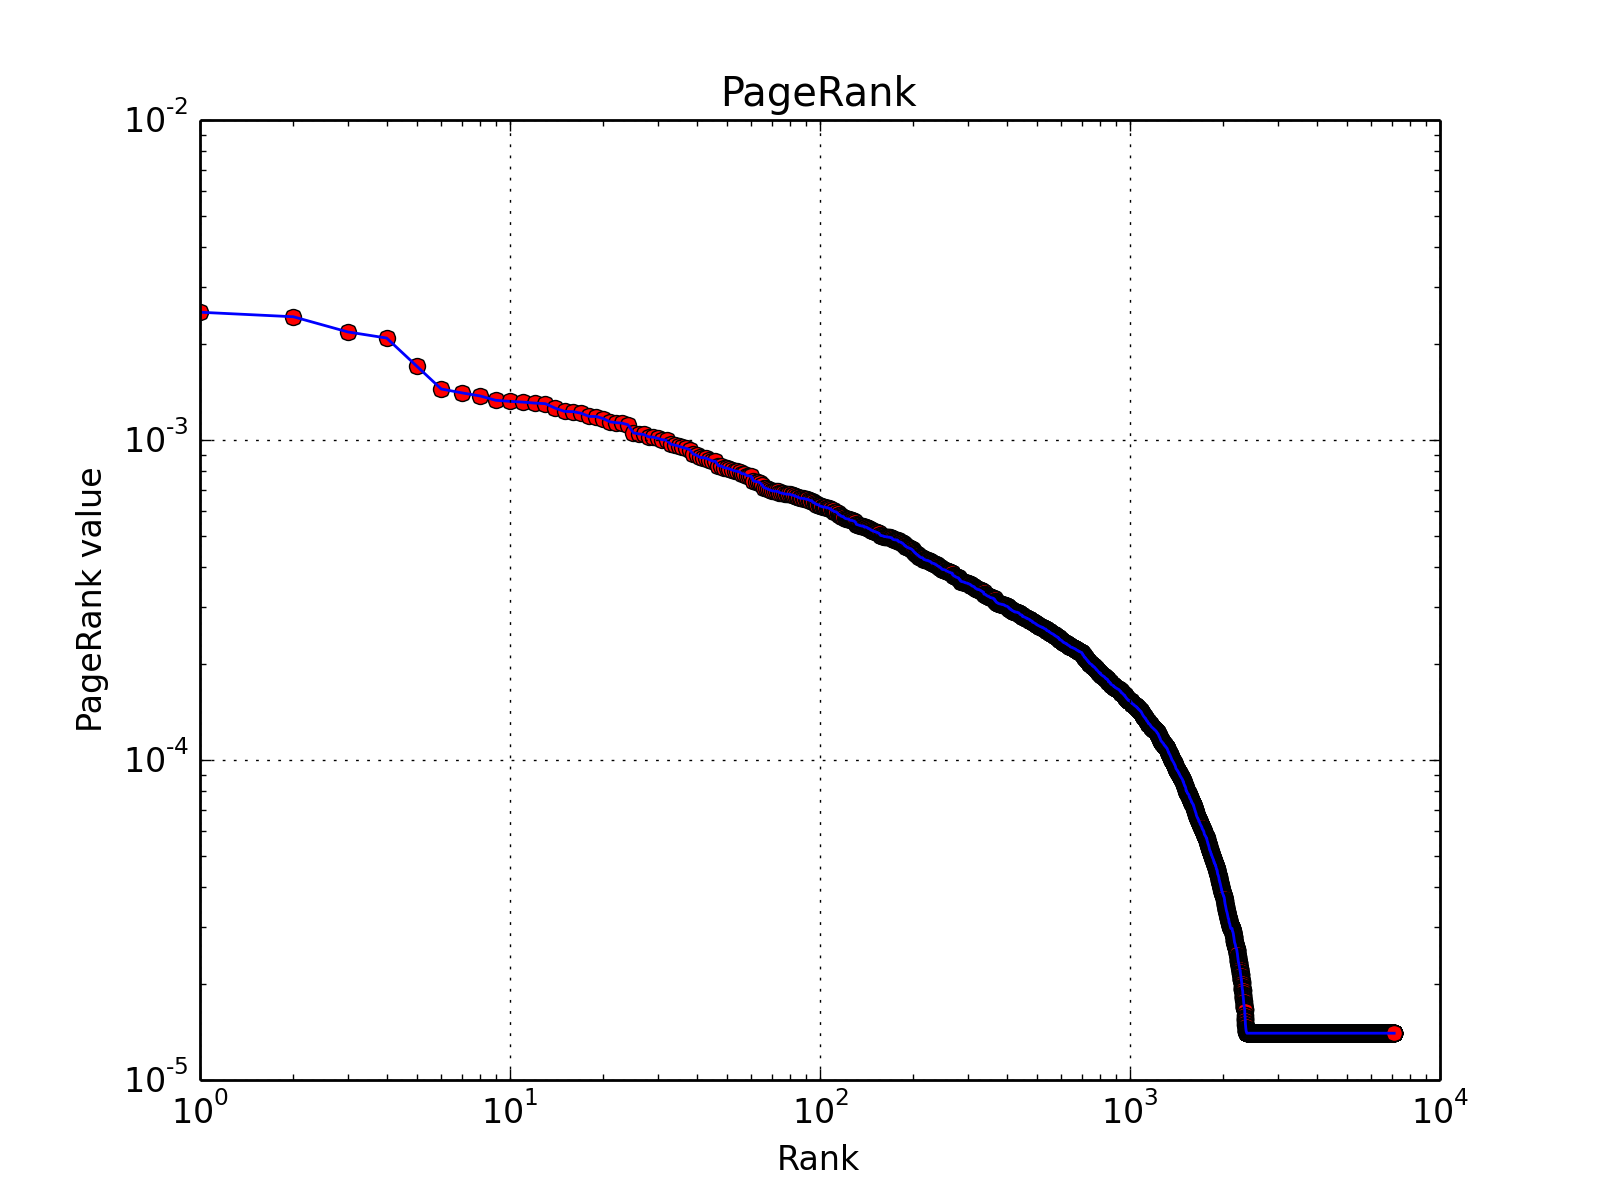
\includegraphics[width=0.5\textwidth]{FIG/pageRankoutput_wiki-Vote.png} 
\end{tabular}
\caption{PageRank of soc(left) and Wiki(right)}
\label{fig:results}
\end{center}
\end{figure}

\subsection{Connected Component}

\par Connected component before K-core decomposition: \\
\par \textbf{(a) soc-Epinions1}
\par Component Number: 2
\begin{itemize}
\item Component 1: 75877 nodes
\item Component 2: 2 nodes
\end{itemize}

\par \textbf{(b) wiki-Vote}
\par Component Number: 24
\begin{itemize}
\item 20 components of 2 nodes
\item 3 components of 3 nodes
\item 1 component of 7066 nodes
\end{itemize}

\subsection{KCore}

\par After running kcore, the results for the two datasets are: \\
\par \textbf{(a) soc-Epinions1}
\par Number of coreness=5 nodes : 19241
\par 1 weakly connected component in total Component 1: 19241 nodes\\

\par \textbf{(b) wiki-Vote}
\par Number of coreness=5 nodes : 3513
\par 1 weakly connected component in total Component 1: 3513 nodes